% !TEX root = ../my-thesis.tex

\lstset{breaklines=true, breakatwhitespace=false}

\chapter{Evaluation auf dem HPC-System MOGON}
\label{sec:mogon}
\section{Zielsetzung}
\label{sec:mogon:ziel}

Die lokale Evaluation in Kapitel~\ref{sec:lokal} betrachtet die fünf
Systeme unter kontrollierten Bedingungen auf einem einzelnen
Rechner. Damit ist die Frage, wie sich dieselben Systeme in einer
HPC-Umgebung einsetzen lassen, noch nicht beantwortet. Ein
HPC-System unterscheidet sich in zwei Punkten von einem einzelnen
Rechner. Die Software muss unter den Rechten eines gewöhnlichen
Nutzerkontos bereitgestellt werden, ohne Administrationsrechte.
Die Ausführung der Rechenschritte erfolgt nicht unmittelbar,
sondern über einen Ressourcenverwalter, der die Rechenknoten
zwischen allen Nutzenden aufteilt.

Dieses Kapitel untersucht deshalb zunächst, mit welchem Aufwand
sich die Systeme auf dem HPC-System MOGON bereitstellen lassen und
wie sie ihre Rechenschritte an den Ressourcenverwalter Slurm
übergeben. Darauf aufbauend wird betrachtet, welche Zeitanteile
eines Laufs im regulären Clusterbetrieb entstehen und woher sie
stammen. Aus dieser Betrachtung ergibt sich der Aufbau der
anschließenden Messung, deren Ergebnisse den letzten Teil des
Kapitels bilden.

Workflows, Benchmark-Skripte, Instrumentierung und Messgrößen sind
dieselben wie in Kapitel~\ref{sec:methodik} beschrieben, ebenso die
Referenzmessung ohne Workflow-Management-System und die fünf
beziehungsweise drei Wiederholungen je Konfiguration, über die die
Messwerte zusammengefasst werden. Da sich die
Ausführungsbedingungen beider Ebenen unterscheiden, werden die
Ergebnisse getrennt betrachtet und nicht unmittelbar
gegeneinander gestellt.


\section{Versuchsumgebung}
\label{sec:mogon:umgebung}

Die Untersuchung wurde auf dem HPC-System MOGON NHR Süd-West der
Johannes Gutenberg-Universität Mainz durchgeführt, das aus 590
Rechenknoten mit insgesamt rund 75.000 Rechenkernen
besteht~\cite{mogonnhr}. Der Zugang erfolgt über einen
Login-Knoten, auf dem Software eingerichtet und Rechenaufträge
eingereicht werden. Die eigentliche Ausführung findet auf
Rechenknoten statt, die der Ressourcenverwalter Slurm in der
Version 24.11.6 zuteilt.

Alle Läufe wurden in der Partition \texttt{ki-smallcpu} ausgeführt,
die 29 gleichartige Rechenknoten umfasst. Ein Knoten dieser
Partition besitzt zwei Prozessoren des Typs AMD EPYC 7713 mit je 64
Kernen~\cite{mogonnhr}, insgesamt 128 Rechenkerne und 248~GB
Hauptspeicher. Als Betriebssystem kommt AlmaLinux 8.10 zum Einsatz.

Für die Datenhaltung stehen zwei Ablageorte zur Verfügung. Das
gemeinsame Dateisystem \texttt{/fshpc} ist über NFS eingebunden und von allen Knoten aus erreichbar. Zusätzlich
verfügt jeder Rechenknoten über einen lokalen Zwischenspeicher, der
einem Rechenauftrag für dessen Laufzeit unter
\texttt{/localscratch} zugewiesen und nach dessen Ende verworfen
wird. Dieser Speicher ist nur innerhalb des jeweiligen Knotens
sichtbar. Die Benchmark-Workflows und ihre Arbeitsverzeichnisse
lagen im gemeinsamen Dateisystem, da Workflow-Schritte auf
unterschiedlichen Rechenknoten ausgeführt werden können und ihre
Zwischenergebnisse deshalb über einen von allen Knoten
erreichbaren Speicher austauschen müssen.

Software wird auf dem Cluster über ein Modulsystem bereitgestellt,
über das sich vorinstallierte Pakete in die eigene Umgebung laden
lassen~\cite{mogondocs}, darunter Python in der Version 3.12.3 und
Apptainer in der Version 1.3.4. Welche der untersuchten Systeme
darüber verfügbar waren und wie die übrigen eingerichtet wurden,
beschreibt Abschnitt~\ref{sec:mogon:bereitstellung}.


\section{Bereitstellung und Betrieb der Systeme}
\label{sec:mogon:bereitstellung}

Die folgenden Abschnitte beschreiben je System, wie es auf MOGON
bereitgestellt wurde, welche Bestandteile der lokalen Umsetzung
übernommen werden konnten, welche Anpassungen für die Ausführung
über Slurm erforderlich waren und wie ein Lauf betrieben wird.
\subsection{Nextflow}
\label{sec:mogon:nextflow}

Nextflow steht auf MOGON als Modul zur Verfügung und wird mit
\texttt{module load tools/Nextflow/25.10.4} in die eigene Umgebung
geladen. Damit ist die Bereitstellung abgeschlossen. Das Modul
bringt die benötigte Java-Laufzeitumgebung bereits mit. Wie in der
lokalen Untersuchungsumgebung
(Abschnitt~\ref{sec:lokal:umgebung}) benötigt Nextflow auch auf
MOGON keine zusätzlichen Dienste oder dauerhaft laufenden
Hintergrundprozesse.

Die Workflow-Beschreibungen beider Muster wurden unverändert aus der lokalen Umsetzung übernommen. Zusätzlich wurde eine Konfigurationsdatei
\texttt{nextflow.config} verwendet.
Während Nextflow die Schritte in der lokalen Ausführungsumgebung unmittelbar als Prozesse auf dem ausführenden Rechner startet, legt die Konfigurationsdatei auf dem Cluster fest, dass die Ausführung über Slurm erfolgt und mit welchen Ressourcen die einzelnen Workflow-Schritte angefordert werden.

Listing~\ref{lst:mogon:nfconfig} zeigt die verwendete
Konfiguration. Die Zeile \texttt{executor = 'slurm'} legt fest, dass Nextflow die Workflow-Schritte über Slurm ausführt, alle weiteren Angaben betreffen die einzelnen Slurm-Jobs. Partition und Konto werden an Slurm übergeben, die
Angaben zu Rechenkernen, Hauptspeicher und Zeitlimit gelten je
Schritt und nicht für den Workflow als Ganzes. Der Eintrag
\texttt{queueSize} begrenzt darüber hinaus, wie viele Jobs Nextflow
gleichzeitig bei Slurm einreicht. 

\begin{lstlisting}[language=Java,
  caption={Konfiguration von Nextflow für die Ausführung auf MOGON},
  label={lst:mogon:nfconfig}]
process {
    executor = 'slurm'
    queue = 'ki-smallcpu'
    clusterOptions = '-A ki-mawahpc'
    cpus = 1
    memory = '1 GB'
    time = '00:10:00'
}
executor {
    queueSize = 4
}
\end{lstlisting}

Gestartet wird ein Lauf mit einem einzelnen Aufruf von
\texttt{nextflow run} auf dem Login-Knoten. Der dabei entstehende
Vordergrundprozess übernimmt die Steuerung des Workflows, reicht die
Schritte bei Slurm ein und überwacht deren Ausführung. Mit dem Ende
dieses Prozesses ist der Lauf abgeschlossen, es bleibt kein Dienst
zurück. Bei Einrichtung und Betrieb traten keine Fehler auf.


\subsection{StreamFlow}
\label{sec:mogon:streamflow}

StreamFlow steht auf MOGON nicht als Modul zur Verfügung und wurde
deshalb in einer eigenen Conda-Umgebung installiert.
Zum Einsatz kommt die Version 0.2.0rc2. Wie in der lokalen
Untersuchungsumgebung (Abschnitt~\ref{sec:lokal:umgebung}) benötigt
StreamFlow auch auf MOGON keine zusätzlichen Dienste.

Die Workflow-Beschreibungen beider Muster wurden unverändert aus der 
lokalen Umsetzung übernommen. Zusätzlich wurde die Datei \texttt{streamflow.yml} angepasst. Während sie in der lokalen Ausführungsumgebung ein Deployment vom Typ \texttt{local} verwendet,
das die Workflow-Schritte unmittelbar als Prozesse auf dem ausführenden Rechner startet, legt sie auf dem Cluster fest, dass die Ausführung über Slurm erfolgt und mit welchen Ressourcen die einzelnen Workflow-Schritte angefordert werden.

Listing~\ref{lst:mogon:sfconfig} zeigt einen Auszug aus der
Umgebungsbeschreibung. Der Eintrag \texttt{bindings} ordnet die
Schritte des Workflows dem Deployment \texttt{slurm-mogon} zu.
Dessen Angaben zu Partition, Konto, Rechenkernen, Hauptspeicher und
Zeitlimit gelten je Schritt und nicht für den Workflow als Ganzes.
Der Eintrag \texttt{maxConcurrentJobs} begrenzt darüber hinaus, wie
viele Jobs StreamFlow gleichzeitig bei Slurm einreicht. Über
\texttt{wraps} ist festgelegt, dass das Slurm-Deployment auf dem
lokalen Deployment \texttt{mogon-local} aufbaut, über das die
Slurm-Kommandos vom Login-Knoten aus ausgeführt werden. Der Eintrag
\texttt{workdir} legt fest, in welchem Verzeichnis StreamFlow die
Arbeitsverzeichnisse der einzelnen Workflow-Schritte anlegt.
Voreingestellt ist \texttt{/tmp}, das auf jedem Rechenknoten
getrennt existiert. Für die Ausführung auf MOGON wurde stattdessen
das gemeinsame Dateisystem \texttt{/fshpc} verwendet, da
Workflow-Schritte auf unterschiedlichen Rechenknoten ausgeführt
werden können und die erzeugten Dateien allen nachfolgenden
Schritten zur Verfügung stehen müssen.

\begin{lstlisting}[language=Python,
  caption={Auszug aus der Umgebungsbeschreibung von StreamFlow für die Ausführung auf MOGON},
  label={lst:mogon:sfconfig}]
    bindings:
      - step: /
        target:
          deployment: slurm-mogon
          service: default

deployments:
  mogon-local:
    type: local
    workdir: /fshpc/antahiri/slurm_modus/streamflow/pipeline/workdir
    config: {}

  slurm-mogon:
    type: slurm
    wraps: mogon-local
    workdir: /fshpc/antahiri/slurm_modus/streamflow/pipeline/workdir
    config: 
      maxConcurrentJobs: 4
      services:
        default:
          account: ki-mawahpc
          partition: ki-smallcpu
          nodes: "1"
          ntasks: 1
          cpusPerTask: 1
          mem: "1G"
          time: "00:10:00"
\end{lstlisting}

Eine weitere Anpassung betraf StreamFlow selbst. Um den Zustand
eines eingereichten Jobs zu verfolgen, ruft StreamFlow die
Slurm-Kommandos \texttt{scontrol} und \texttt{squeue} mit der
Kennung des Jobs auf. MOGON ist als Verbund mehrerer Cluster
eingerichtet, und beim Einreichen eines Jobs wird neben der Nummer
auch der ausführende Cluster zurückgemeldet. StreamFlow führte
beide Angaben zu einer Kennung der Form \texttt{454783;mogonki}
zusammen und gab diese unverändert an die Abfragen weiter, die
daraufhin kein Ergebnis lieferten. Die Anpassung in der Datei
\texttt{queue\_manager.py} entfernt den angehängten Clusternamen,
bevor die Kennung verwendet wird. Dabei ist zu berücksichtigen,
dass es sich bei Version 0.2.0rc2 um eine Vorabversion handelt.

Gestartet wird ein Lauf mit einem einzelnen Aufruf von
\texttt{streamflow run} auf dem Login-Knoten. Der dabei entstehende
Vordergrundprozess übernimmt die Steuerung des Workflows, reicht die
Schritte bei Slurm ein und überwacht deren Ausführung. Mit dem Ende
dieses Prozesses ist der Lauf abgeschlossen, es bleibt kein Dienst
zurück.

\subsection{Merlin}
\label{sec:mogon:merlin}

Merlin steht auf MOGON nicht als Modul zur Verfügung und wurde
deshalb in einer eigenen Conda-Umgebung installiert. Zum Einsatz
kommt dieselbe Version 1.13.0 wie in der lokalen
Untersuchungsumgebung (Abschnitt~\ref{sec:lokal:umgebung}). Wie
bereits dort beschrieben, benötigt Merlin zusätzlich einen
Redis-Server. Da auf dem Cluster kein Docker zur Verfügung steht,
wurde Redis über einen Apptainer-Container bereitgestellt, der sich
mit den Rechten eines gewöhnlichen Nutzerkontos ausführen lässt.
Die Verbindungsdaten zum Redis-Server stehen in der Datei
\texttt{app.yaml} im Nutzerverzeichnis, deren Servereintrag auf den
Ort zeigt, an dem Redis für den jeweiligen Lauf gestartet wird.

Die Workflow-Beschreibungen beider Muster wurden unverändert aus der
lokalen Umsetzung übernommen. Hinzu kam für den Betrieb auf dem
Cluster das Slurm-Jobskript \texttt{worker\_job.sbatch}, mit dem die
Worker bei Slurm eingereicht werden.

Listing~\ref{lst:mogon:merlinjob} zeigt das verwendete
Slurm-Jobskript. Der obere Teil fordert die Ressourcen für den
Worker-Job bei Slurm an, darunter Partition, Konto,
Rechenkerne, Hauptspeicher und Zeitlimit. Anders als bei Nextflow
und StreamFlow gelten diese Angaben nicht für einzelne
Workflow-Schritte, sondern für die gesamte Allokation, in der die
Worker ausgeführt werden. Der untere Teil bereitet die Umgebung vor
und startet den Celery-Worker.

\begin{lstlisting}[language=bash,
  caption={Jobskript zum Start der Merlin-Worker auf MOGON},
  label={lst:mogon:merlinjob}]
#!/bin/bash
#SBATCH --account=ki-mawahpc
#SBATCH --job-name=merlin-worker-pipeline
#SBATCH --partition=ki-smallcpu
#SBATCH --nodes=1
#SBATCH --ntasks=1
#SBATCH --cpus-per-task=1
#SBATCH --mem=2G
#SBATCH --time=00:15:00
#SBATCH --output=worker_%j.out

module purge
module load lang/Anaconda3/2024.06-1
conda activate merlin2
cd ~/slurm_modus/merlin/pipeline

export LANG=C LC_ALL=C

celery -A merlin worker \
  --concurrency 1 \
  --prefetch-multiplier 1 \
  -O fair \
  -l INFO \
  -n beobachtung_worker.%h \
  -Q "[merlin]_merlin"
\end{lstlisting}

Ein Lauf wird auf dem Cluster mit zwei Befehlen gestartet. Der Aufruf von \texttt{merlin run} bereitet die Ausführung des
Workflows vor und übergibt die auszuführenden Aufgaben an den
Nachrichtenvermittler und kehrt danach zurück. Getrennt
davon wird das Jobskript mit \texttt{sbatch} eingereicht, woraufhin
die Worker die Aufgaben abarbeiten. Der Worker-Job endet nicht von
selbst, sondern muss nach dem Lauf beendet werden. Auch der
Redis-Server bleibt danach aktiv. 

Bei der Einrichtung trat derselbe Fehler auf wie in der lokalen Umgebung. Das von Merlin vorausgesetzte Modul \texttt{pkg\_resources} fehlt in aktuellen
Versionen von \texttt{setuptools}, sodass ein Downgrade nötig war.


\subsection{Pegasus}
\label{sec:mogon:pegasus}

Pegasus setzt für die Ausführung der geplanten Workflows HTCondor
voraus, an dessen Warteschlange die einzelnen Aufgaben übergeben
werden. HTCondor stand auf MOGON nicht als Systemsoftware zur Verfügung.
Für HPC-Systeme beschreibt die Dokumentation neben einer
Installation durch die Administration, die allen Nutzenden zur
Verfügung steht, auch eine nutzerseitige Installation, bei der
HTCondor auf dem Login-Knoten betrieben wird~\cite{pegasusdocs}.

Der dafür vorgesehene Bezugsweg war auf MOGON nicht nutzbar, da die
Downloadadressen über den Proxy des Rechenzentrums nicht erreichbar
waren. Eine Installation über Conda stellte lediglich
Clientwerkzeuge und Python-Komponenten bereit, nicht jedoch die für
den Betrieb erforderlichen HTCondor-Dienste. Damit stand für die
geplante Ausführung keine funktionsfähige HTCondor-Installation zur
Verfügung.

Pegasus konnte daher in die nachfolgenden Untersuchungen nicht einbezogen werden.

\subsection{AiiDA}
\label{sec:mogon:aiida}
AiiDA steht auf MOGON nicht als Modul zur Verfügung und wurde
deshalb in einer eigenen Conda-Umgebung installiert. Zum Einsatz
kommt dieselbe Version 2.8.0 wie in der lokalen
Untersuchungsumgebung (Abschnitt~\ref{sec:lokal:umgebung}). Wie bereits dort beschrieben, verwendet die empfohlene Konfiguration von AiiDA PostgreSQL als Datenbank und RabbitMQ für die Kommunikation mit dem Daemon~\cite{aiidadocs-install}. Beide Dienste lassen sich mit den Rechten eines gewöhnlichen
Nutzerkontos betreiben, RabbitMQ wurde über dieselbe Conda-Umgebung
installiert. Welche Datenbank ein Profil verwendet, wird bei der Einrichtung
festgelegt. Auf die Auswirkungen der verschiedenen
Konfigurationen geht Abschnitt~\ref{sec:mogon:konfigstudie} ein.

Die WorkChains beider Muster wurden aus der lokalen Umsetzung
übernommen und um die Angaben ergänzt, mit denen die einzelnen
Aufgaben bei Slurm eingereicht werden, darunter Partition, Konto
und Zeitlimit. Profil, Rechner- und Code-Eintrag wurden wie in der
lokalen Umgebung angelegt, mit zwei Änderungen im Rechner-Eintrag:
Als Scheduler ist \texttt{core.slurm} statt \texttt{core.direct}
eingetragen, wodurch AiiDA die Aufgaben als Slurm-Jobs einreicht,
und das Arbeitsverzeichnis liegt auf dem gemeinsamen Dateisystem.

Listing~\ref{lst:mogon:aiidacomputer} zeigt den Rechner-Eintrag, der
für die Ausführung über Slurm angelegt wurde. Die Angaben zu
Partition, Konto und Zeitlimit stehen nicht in diesem Eintrag,
sondern in den WorkChains, bei dem jeweiligen Prozess. Der Transport
\texttt{core.local} legt fest, dass die Kommandos auf dem
Login-Knoten ausgeführt werden, der Scheduler \texttt{core.slurm}
bestimmt, dass AiiDA für jede Aufgabe ein Jobskript erzeugt und
dieses bei Slurm einreicht. Das Arbeitsverzeichnis liegt auf dem
gemeinsamen Dateisystem. 

\begin{lstlisting}[
  caption={Rechner-Eintrag und Ressourcenangaben für die Ausführung über Slurm},
  label={lst:mogon:aiidacomputer}]
Label                        mogon-slurm
Transport type               core.local
Scheduler type               core.slurm
Work directory               /fshpc/antahiri/slurm_modus/aiida/work
Default #procs/machine       1

# Ressourcenangaben je Aufgabe in der WorkChain
"queue_name": "ki-smallcpu",
"account": "ki-mawahpc",
"max_wallclock_seconds": 600,
"resources": {"num_machines": 1, "num_mpiprocs_per_machine": 1},
\end{lstlisting}

Ein Lauf wird über ein kurzes Python-Skript eingereicht, das die
Eingaben als Knoten anlegt und die WorkChain an den Daemon
übergibt. Damit dessen Worker die WorkChain-Klassen laden können, muss das Verzeichnis, das diese Klassen enthält, im Suchpfad von Python liegen, bevor der Daemon gestartet wird, da er seine Umgebung nur beim Start übernimmt. Nach dem Einreichen kehrt das Skript zurück und der
Daemon führt den Workflow im Hintergrund aus. Daemon und
Nachrichtenvermittler laufen dabei unabhängig von der Sitzung
weiter.


\section{Ausführung im Slurm-Betrieb}
\label{sec:mogon:slurmbetrieb}

Alle vier verbleibenden Systeme führen ihre Workflow-Schritte über
Slurm aus, unterscheiden sich jedoch darin, wie sie den
Ressourcenverwalter in die Ausführung einbinden. Bei Nextflow und
StreamFlow reicht der Vordergrundprozess auf dem Login-Knoten für
jeden Workflow-Schritt einen eigenen Slurm-Job ein, beobachtet deren Zustand durch wiederholte Abfragen und reicht abhängige
Schritte erst ein, wenn ihre Vorgänger abgeschlossen sind. Ein Lauf
mit neun Schritten erzeugt so neun Slurm-Jobs, die
jeweils Warteschlange und Prolog durchlaufen, bevor die eigentliche
Ausführung beginnt.

Bei AiiDA übernimmt der Daemon diese Aufgabe. Er erzeugt für jede
Aufgabe ein Jobskript, reicht dieses bei Slurm ein und fragt den
Zustand der Jobs zyklisch ab. Der Unterschied zu Nextflow und
StreamFlow liegt nicht im Umgang mit Slurm, sondern darin, dass die
Steuerung nicht an einen Vordergrundprozess gebunden ist. Das
einreichende Skript kehrt unmittelbar zurück, während der Daemon
den Workflow unabhängig von der Sitzung fortführt.

Merlin bindet Slurm auf andere Weise ein. Statt je Schritt einen
Job einzureichen, wird ein einziger Job gestartet, dessen
Allokation für die gesamte Dauer des Laufs bestehen bleibt. In dieser Allokation laufen die Worker, die sich die Aufgaben aus der Warteschlange
holen und abarbeiten. Warteschlange und Prolog fallen dadurch
einmal je Lauf an statt einmal je Schritt und aufeinanderfolgende Schritte starten ohne erneuten Weg über den
Ressourcenverwalter. Dieses Modell nutzt das Prinzip eines Pilot-Jobs: Ein Platzhalter-Job belegt die Ressourcen, und mehrere Aufgaben werden innerhalb seiner Laufzeit ausgeführt, wodurch die je Job anfallenden Scheduling-Anteile entfallen~\cite{chen2011overhead}.

Aus diesen Ausführungsmodellen ergibt sich die Frage, wie sich die
Laufzeit eines Workflows im regulären Clusterbetrieb
zusammensetzt. Dazu wurden Beobachtungsläufe durchgeführt, zunächst
mit Nextflow, bei dem beide Workflow-Muster in fünf Wiederholungen
ausgeführt wurden. Für jeden Slurm-Job wurde die Zeit vom
Einreichen bis zum Ende der Nutzlast in drei Anteile zerlegt: Die
Wartezeit in der Warteschlange, die Zeit zwischen dem Start des
Jobs und dem ersten Zeitstempel der Nutzlast, sowie die Laufzeit
der Nutzlast selbst. Die ersten beiden Anteile wurden aus den
Zeitstempeln von \texttt{sacct} bestimmt, die Laufzeit der Nutzlast
aus den Zeitmessungen der Benchmark-Skripte. Die getrennte Betrachtung verschiedener Zeitanteile folgt dem in Abschnitt~\ref{sec:methodik:messgroessen} beschriebenen Vorgehen
von Chen und Deelman~\cite{chen2011overhead}.

\begin{figure}[htbp]
  \centering
  \begin{subfigure}{0.80\textwidth}
    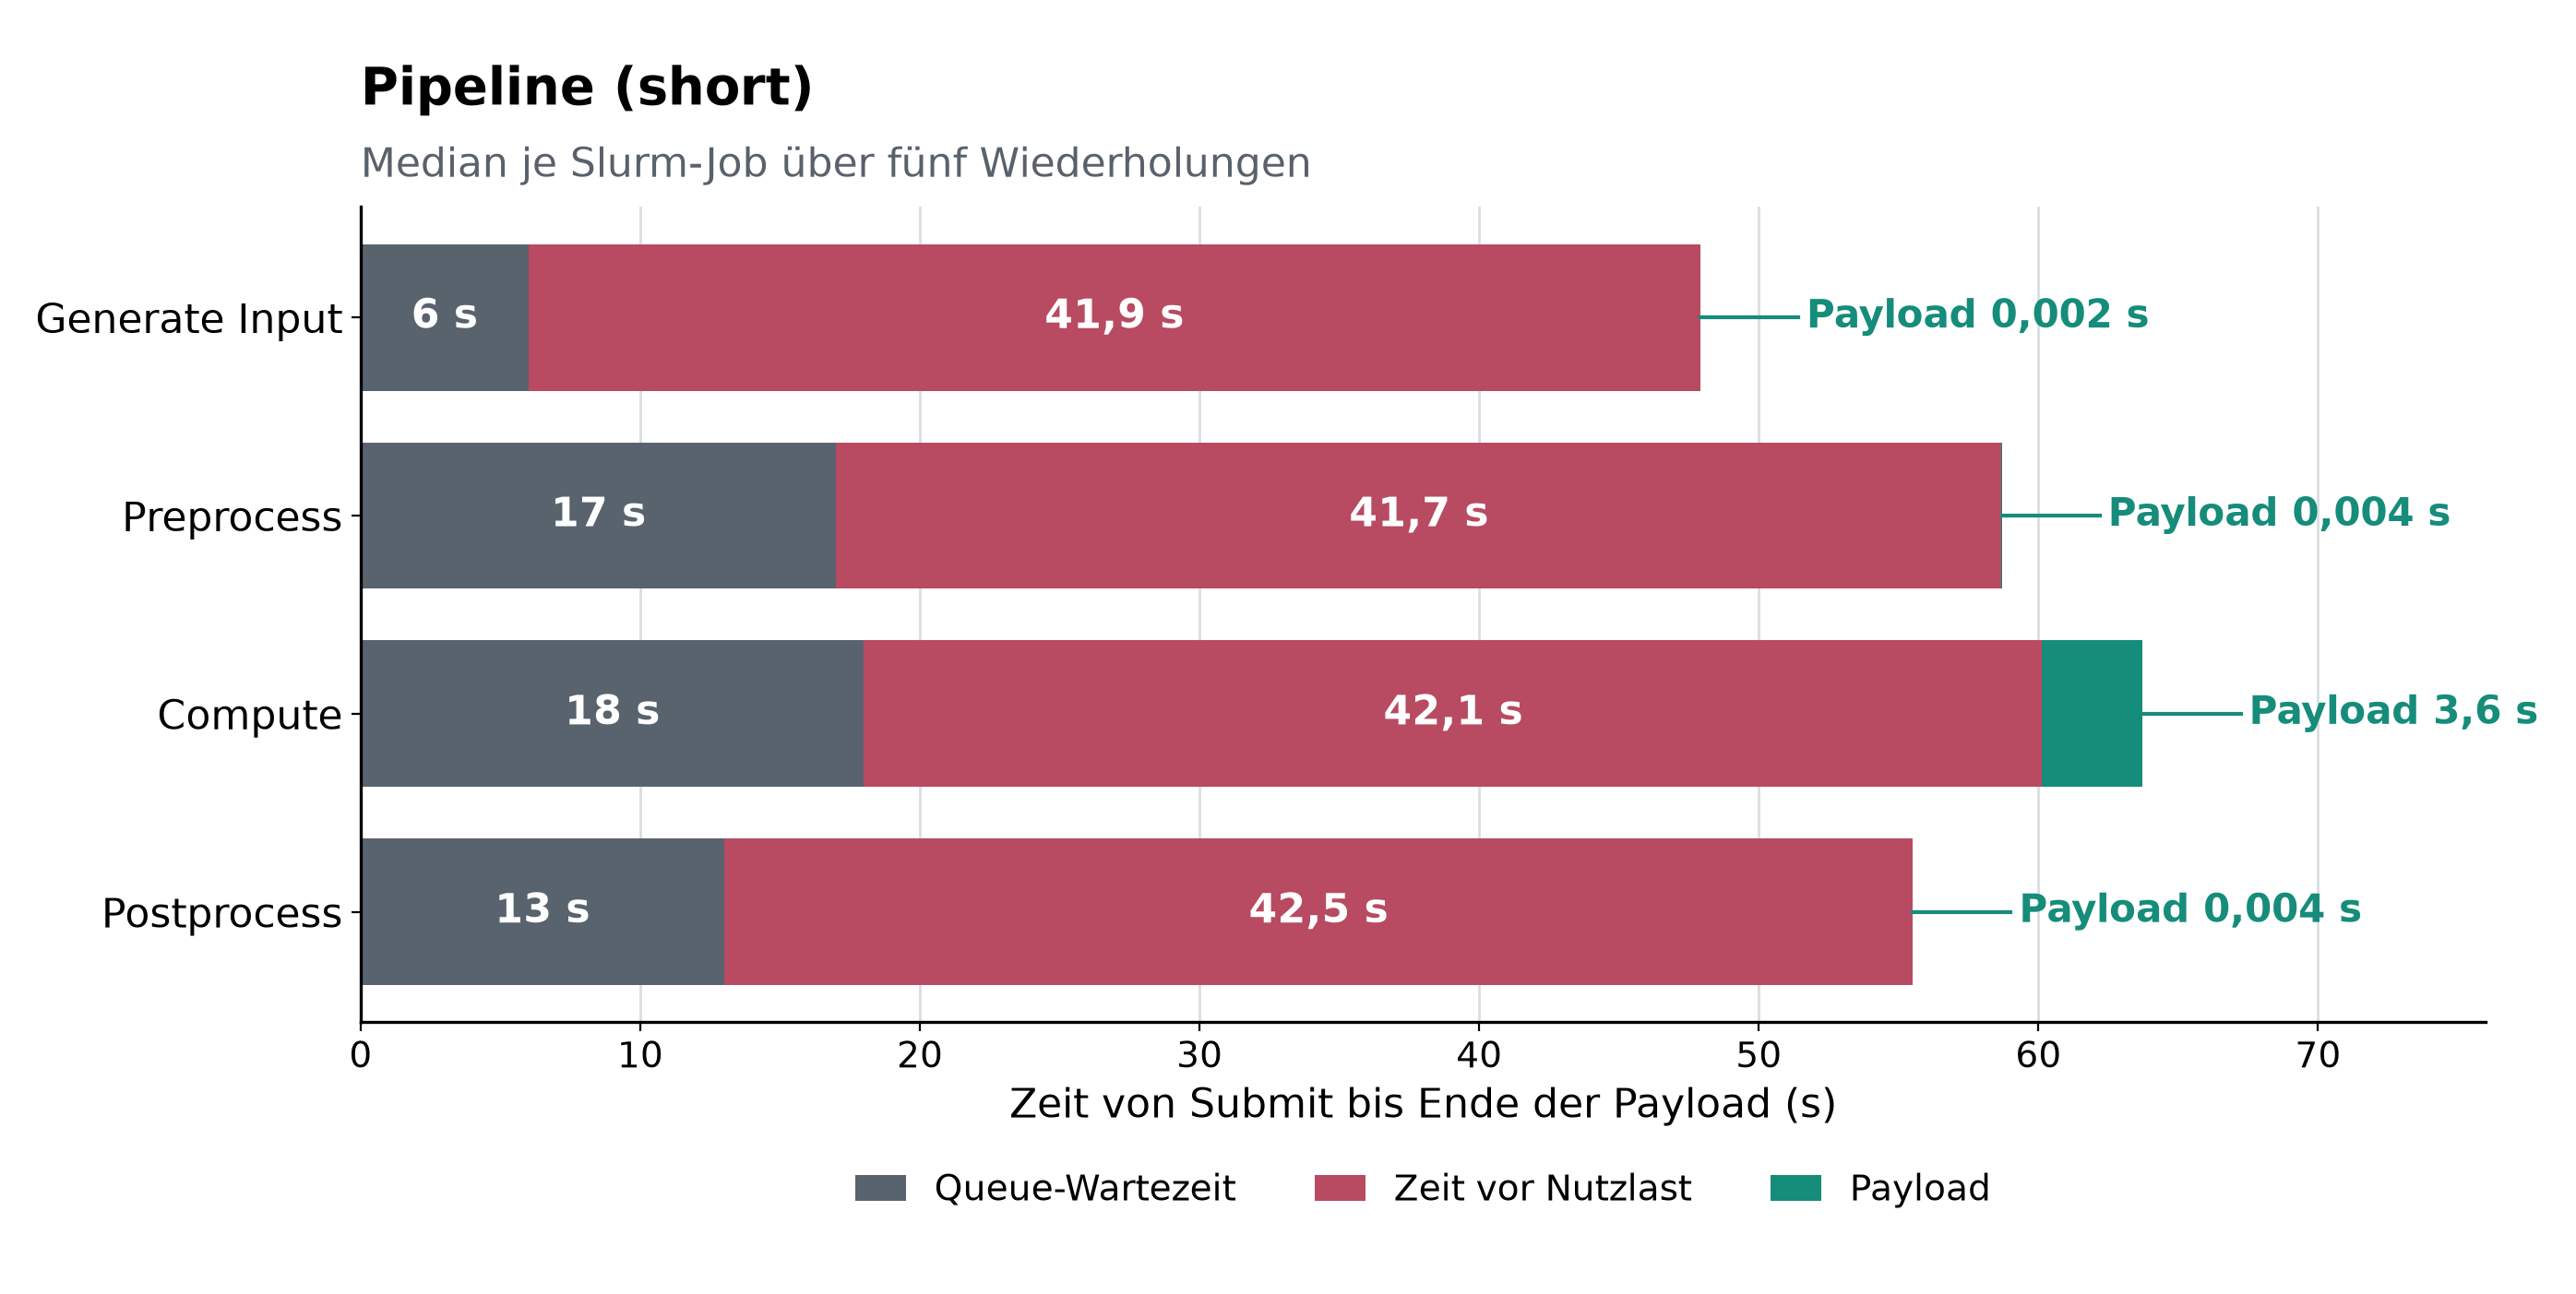
\includegraphics[width=\textwidth]{content/figs/Zerlegungen/abb_pipeline_zerlegung.png}
    \caption{Pipeline-Muster}
    \label{fig:mogon:zerlegung-pipeline}
  \end{subfigure}\\[2ex]
  \begin{subfigure}{0.80\textwidth}
    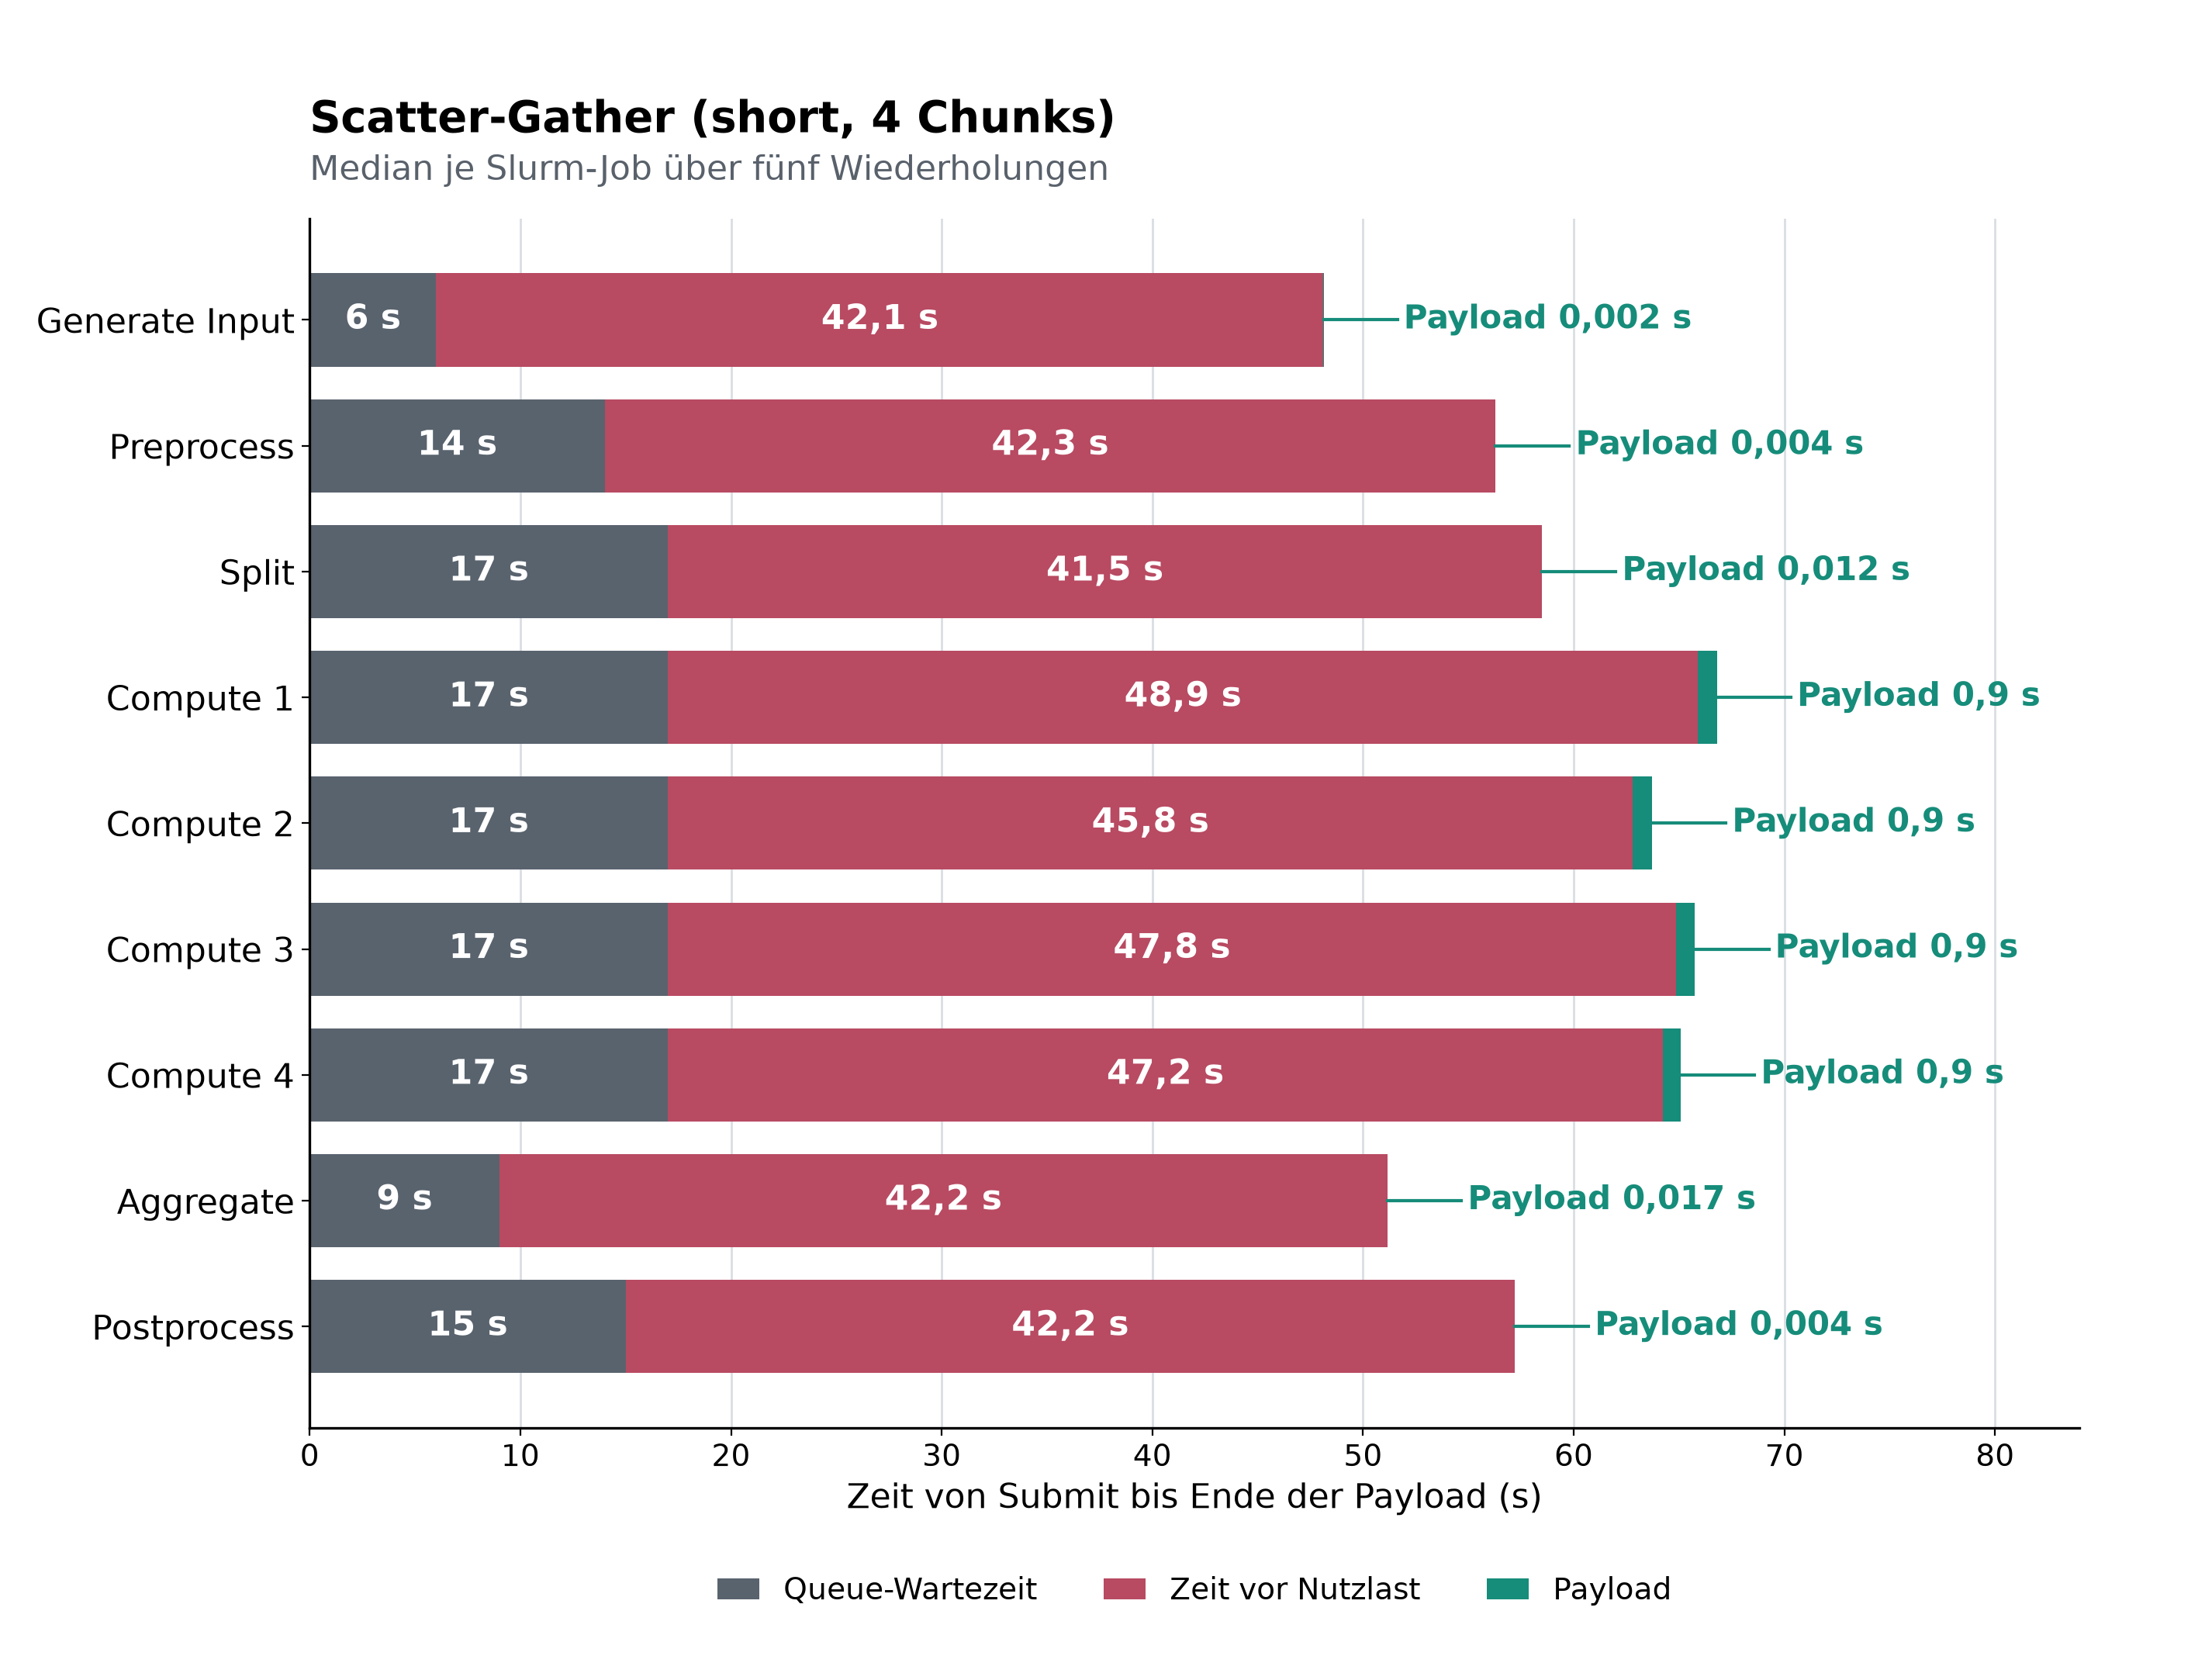
\includegraphics[width=\textwidth]{content/figs/Zerlegungen/abb_scatter_gather_zerlegung.png}
    \caption{Scatter-Gather-Muster mit vier Chunks}
    \label{fig:mogon:zerlegung-sg}
  \end{subfigure}
  \caption{Zerlegung der Zeit vom Einreichen bis zum Ende der
    Nutzlast je Slurm-Job, Median über fünf Wiederholungen mit
    Nextflow.}
  \label{fig:mogon:zerlegung}
\end{figure}

Die Abbildungen~\ref{fig:mogon:zerlegung-pipeline} und~\ref{fig:mogon:zerlegung-sg} zeigen die Zerlegung für beide Muster. Die Laufzeit der Nutzlast liegt bei den meisten Schritten im
Millisekundenbereich und ist in den Balken daher kaum sichtbar.
Lediglich die Compute-Schritte erreichen mit 3,6 beziehungsweise
0,9 Sekunden nennenswerte Werte. Die Wartezeit in der Warteschlange
schwankt zwischen 6 und 17 Sekunden. Der mittlere Anteil liegt
dagegen durchgehend bei über 40 Sekunden je Job und stellt damit
den mit Abstand größten Zeitanteil dar. Auffällig ist zudem, dass dieser Anteil auch
zwischen gleichartigen Jobs schwankt: Die vier Compute-Jobs des
Scatter-Gather-Musters wurden gleichzeitig eingereicht und warteten
gleich lange, ihr mittlerer Anteil reicht dennoch von 45,8 bis
48,9 Sekunden.

Dieser mittlere Anteil wird hier bewusst nicht als Prolog
bezeichnet, denn er umfasst zwei Dinge: die Arbeiten, die der
Cluster vor dem Start des Jobskripts ausführt, und die Schritte,
die das Workflow-Management-System innerhalb des Jobs erledigt,
bevor die Nutzlast beginnt. Aus der Zerlegung allein ist nicht
ersichtlich, wie sich der Anteil auf den Cluster und das Workflow-Management-System verteilt.
\FloatBarrier

Um diese Aufteilung näher zu untersuchen, wurde der zuvor bestimmte mittlere Zeitanteil anschließend für alle vier Systeme gesondert untersucht. Dazu wurde je System analysiert, welche Schritte nach der Übergabe des Slurm-Jobs an das erzeugte Jobskript und vor dem ersten Zeitstempel der Nutzlast
ausgeführt werden. Da sich Aufbau und Ablauf der Jobskripte
zwischen den Systemen unterscheiden, erfolgte diese Untersuchung
systemspezifisch.

Der so bestimmte Anteil liegt bei den drei Systemen, die Jobs je
Schritt einreichen, im Bereich von 55 bis 104 Millisekunden. Damit liegt der systemeigene Anteil um mehrere Größenordnungen unter dem zuvor beobachteten mittleren Zeitanteil von über 40 Sekunden je Job. Bei
Merlin entsteht ein vergleichbarer Aufwand nicht je
Workflow-Schritt, sondern einmal beim Start der Worker-Allokation.


Die Zerlegung zeigt damit, dass der systemeigene Anteil im
Millisekundenbereich liegt und gegenüber den durch den Cluster
verursachten Zeitanteilen vernachlässigbar klein ist. Seine
Bestimmung erfordert zudem systemspezifische Untersuchungen der
jeweiligen Jobabläufe und stellt daher keine einheitliche
Vergleichsgröße dar. Aus diesem Grund wurde der Einfluss des
Clusterbetriebs nicht rechnerisch entfernt, sondern in der
folgenden Messreihe durch eine dedizierte Ausführung experimentell
ausgeschlossen.



\section{Messaufbau der dedizierten Messung}
\label{sec:mogon:dediziert}

Die Messreihen wurden jeweils vollständig innerhalb einer einzelnen
Slurm-Allokation ausgeführt. Dazu wurde ein Rechenknoten der
Partition \texttt{ki-smallcpu} angefordert, auf dem die Systeme
ihre Workflow-Schritte als lokale Prozesse starten, in derselben
Ausführungsform wie in der lokalen Untersuchung in
Kapitel~\ref{sec:lokal}. Warteschlange und Prolog fallen nur beim
Start der jeweiligen Allokation an und liegen vollständig außerhalb
der eigentlichen Messung. Die Ausführung von Benchmark-Messungen
auf dedizierten Rechenknoten entspricht dem Vorgehen vergleichbarer
Untersuchungen~\cite{wfbench2022}.

Dieser Aufbau folgt unmittelbar aus dem Befund des vorangegangenen
Abschnitts. Im regulären Clusterbetrieb entsteht der überwiegende
Teil der Laufzeit durch Warteschlange und die Zeit vor der
Nutzlast, während der systemeigene Anteil im Millisekundenbereich
liegt. Ein Vergleich unter diesen Bedingungen würde deshalb
überwiegend den Zustand des Clusters abbilden. Innerhalb einer
bereits bestehenden Allokation entfallen diese Anteile für die
einzelnen Workflow-Schritte, sodass Unterschiede zwischen den
Systemen nicht mehr durch die je Schritt anfallenden
Warteschlangen- und Prologzeiten überlagert werden.

Workflows, Benchmark-Skripte, Instrumentierung und Messgrößen sind
dieselben wie in Kapitel~\ref{sec:methodik} beschrieben. Auch die
Referenzmessung ohne Workflow-Management-System wurde unverändert
übernommen.

Die Allokation wurde zusätzlich exklusiv angefordert, sodass
während der Messung keine Aufträge anderer Nutzender auf demselben
Knoten liefen. Um den Einfluss dieser Einstellung zu prüfen, wurde
dieselbe Messreihe auch ohne exklusive Reservierung ausgeführt. Die
Unterschiede zwischen beiden Läufen sind gering und nicht
einheitlich gerichtet, bei einzelnen Systemen fielen die Werte auf
dem geteilten Knoten sogar niedriger aus. Die exklusive Messreihe bildet daher die Grundlage der folgenden Auswertung. Die Messung auf dem geteilten Knoten dient ausschließlich dazu, den Einfluss einer geteilten Knotennutzung zu untersuchen.

\begin{figure}[htbp]
  \centering
  \begin{subfigure}{0.49\textwidth}
    
\includegraphics[width=\textwidth]{content/figs/mogon_graphen/05_delta_exklusiv_geteilt_mogon.png}
    \caption{Gesamtlaufzeit}
    \label{fig:mogon:delta-makespan}
  \end{subfigure}
  \hfill
  \begin{subfigure}{0.49\textwidth}
    
\includegraphics[width=\textwidth]{content/figs/mogon_graphen/07_delta_uebergangslatenzen_mogon.png}
    \caption{Übergangslatenzen}
    \label{fig:mogon:delta-latenz}
  \end{subfigure}
  \caption{Differenzen der Mediane zwischen exklusivem und geteiltem
Knoten (exklusiv minus geteilt). Werte nahe null kennzeichnen
geringe Unterschiede zwischen beiden Messreihen.}
  \label{fig:mogon:exklusivgeteilt}
\end{figure}

\section{Ergebnisse der dedizierten Messung}
\label{sec:mogon:ergebnisse}

Berichtet werden dieselben vier Messgrößen wie auf der lokalen
Ebene: die Gesamtlaufzeit, der Overhead gegenüber dem Referenzlauf
sowie die beiden Koordinationsgrößen Übergangslatenz und
Startspreizung. Pegasus ist aus den in
Abschnitt~\ref{sec:mogon:pegasus} genannten Gründen nicht
enthalten, sodass die folgenden Ergebnisse vier Systeme mit jeweils zwölf Konfigurationen umfassen.

Abbildung~\ref{fig:mogon:overhead} stellt den Overhead aller zwölf
Konfigurationen gegenüber. Es bilden sich zwei Gruppen. StreamFlow,
Nextflow und Merlin liegen in zehn der zwölf Konfigurationen
zwischen 1,6 und 4,1 Sekunden und wechseln untereinander die
Reihenfolge. Höhere Werte treten bei den Scatter-Gather-Läufen der
langen Rechenlast mit einem und zwei Teilstücken auf, dort liegen
StreamFlow bei 5,4 und 4,6 Sekunden und Nextflow bei 5,0 und 6,9
Sekunden. AiiDA liegt mit 7,0 bis 14,9 Sekunden in allen zwölf
Konfigurationen über den drei übrigen Systemen.

Ein systemübergreifend einheitlicher Zusammenhang zwischen
Rechenlast und Overhead ist nicht erkennbar, obwohl sich die
Laufzeit der Rechenschritte zwischen der kurzen und der langen
Rechenlast um mehr als das Fünfzigfache unterscheidet. Bei
StreamFlow nimmt der Overhead im Scatter-Gather-Muster zwar mit der
Rechenlast zu, bei den übrigen Systemen zeigt sich diese
Entwicklung jedoch nicht durchgängig.

Bei AiiDA zeigt sich ein Zusammenhang mit dem Umfang
des Workflows. Bei gleicher Rechenlast liegt der Overhead im
Scatter-Gather-Muster durchgängig über dem des Pipeline-Musters.
Zudem steigt er mit der Zahl der Teilstücke. Bei der kurzen
Rechenlast nimmt er von 12,6 Sekunden bei einem Teilstück auf 14,9
Sekunden bei vier Teilstücken zu. Diese Tendenz war bereits auf der lokalen Ebene zu
beobachten, dort stieg der Overhead in derselben Konfiguration von
7,4 auf 9,4 Sekunden.

\begin{figure}[H]
  \centering
  
\includegraphics[width=\textwidth]{content/figs/mogon_graphen/01_overhead_alle_mogon.png}
  \caption{Overhead gegenüber dem Referenzlauf für alle zwölf
    Konfigurationen auf dem HPC-System}
  \label{fig:mogon:overhead}
\end{figure}

Abbildung~\ref{fig:mogon:makespan-pipe} zeigt die Gesamtlaufzeiten
des Pipeline-Musters je Rechenlast. StreamFlow, Nextflow und Merlin
liegen dabei in einem engen Band, bei der kurzen Rechenlast
zwischen 4,9 und 6,7 Sekunden, bei der mittleren zwischen 44,2 und
45,1 Sekunden und bei der langen zwischen 188,4 und 192,1 Sekunden.
AiiDA liegt bei allen drei Rechenlasten darüber, mit 12,3, 56,6 und
229,7 Sekunden. Mit wachsender Rechenlast werden die relativen
Abstände zwischen den Systemen kleiner, da der Overhead gegenüber
der zunehmenden Laufzeit der Rechenschritte an Gewicht verliert.

\begin{figure}[H]
  \centering
  
\includegraphics[width=\textwidth]{content/figs/mogon_graphen/02_makespan_pipeline_mogon.png}
  \caption{Median der Gesamtlaufzeit des Pipeline-Musters je
    Rechenlast auf dem HPC-System, lineare Skala}
  \label{fig:mogon:makespan-pipe}
\end{figure}


Abbildung~\ref{fig:mogon:makespan-sg} zeigt die Gesamtlaufzeiten
des Scatter-Gather-Musters über die Zahl der Teilstücke. Bei der
mittleren und der langen Rechenlast sinken die Laufzeiten mit jeder
Verdopplung der Teilstückzahl deutlich, bei der langen Rechenlast
etwa von 202,2 auf 53,6 Sekunden in StreamFlow und von 223,4 auf
70,4 Sekunden in AiiDA. Bei der kurzen Rechenlast fällt der
Rückgang geringer aus. In StreamFlow, Nextflow und Merlin liegen
die Laufzeiten bei einem Teilstück zwischen 5,3 und 7,1 Sekunden
und bei vier Teilstücken zwischen 3,0 und 4,8 Sekunden. AiiDA
bleibt dort mit 16,4, 15,4 und 16,1 Sekunden über alle
Teilstückzahlen nahezu unverändert.

\begin{figure}[H]
  \centering
  
\includegraphics[width=\textwidth]{content/figs/mogon_graphen/03_makespan_scatter_gather_mogon.png}
  \caption{Median der Gesamtlaufzeit des Scatter-Gather-Musters
    über die Zahl der Teilstücke je Rechenlast auf dem HPC-System}
  \label{fig:mogon:makespan-sg}
\end{figure}

Abbildung~\ref{fig:mogon:latenz} zeigt die Übergangslatenzen
zwischen aufeinanderfolgenden Schritten. Der Median je Übergang
liegt in StreamFlow bei 0,06 Sekunden, in Nextflow bei 0,11, in
Merlin bei 0,14 und in AiiDA bei 1,95 Sekunden, AiiDA liegt damit
etwa um den Faktor 35 über StreamFlow. Innerhalb eines Systems sind
die Werte über die einzelnen Übergänge weitgehend gleich. Erhöht
ist in allen vier Systemen der Übergang vom Verarbeiten zum
Zusammenführen, in StreamFlow 0,14 gegenüber sonst rund 0,06
Sekunden und in AiiDA 2,18 gegenüber rund 1,95 Sekunden. Es ist der
einzige Übergang, an dem die Ergebnisse mehrerer paralleler
Instanzen zusammengeführt werden. Die Übergangslatenz zeigt sich
damit auch auf dem HPC-System als eine weitgehend systemspezifische
Größe, bestimmt von der Stelle, an der ein Schritt an den nächsten
übergeben wird.

\begin{figure}[H]
  \centering
  
\includegraphics[width=\textwidth]{content/figs/mogon_graphen/06_uebergangslatenzen_mogon.png}
  \caption{Median der Übergangslatenzen zwischen aufeinanderfolgenden
    Schritten auf dem HPC-System, logarithmische Skala}
  \label{fig:mogon:latenz}
\end{figure}


Abbildung~\ref{fig:mogon:spreizung} zeigt die Startspreizung der
parallelen Verarbeitungsinstanzen, also den Abstand zwischen dem
ersten und dem letzten Instanzstart. Bei zwei Teilstücken liegt sie
je nach Rechenlast zwischen 3 und 4 Millisekunden in StreamFlow,
zwischen 6 und 7 in Nextflow, zwischen 47 und 50 in Merlin und
zwischen 24 und 32 Millisekunden in AiiDA. Bei vier Teilstücken
liegen die entsprechenden Bereiche bei 18 bis 19, 21 bis 23, 99
bis 114 und 961 bis 1011 Millisekunden. Die Rechenlast beeinflusst
die Startspreizung damit kaum, die Zahl der Teilstücke dagegen
deutlich. In allen vier Systemen wächst sie mit der Zahl der
Teilstücke, am stärksten in AiiDA, wo sie sich von zwei auf vier
Teilstücke mehr als verdreißigfacht.

\begin{figure}[H]
  \centering
  
\includegraphics[width=\textwidth]{content/figs/mogon_graphen/04_startspreizung_mogon.png}
  \caption{Median der Startspreizung der parallelen
    Verarbeitungsinstanzen auf dem HPC-System, logarithmische Skala}
  \label{fig:mogon:spreizung}
\end{figure}

AiiDA weist beim Overhead und bei den Übergangslatenzen die
höchsten Werte auf, bei der Startspreizung mit vier Teilstücken
ebenfalls, bei zwei Teilstücken liegt dort Merlin darüber. Bereits
im Pipeline-Muster summieren sich die drei Übergangslatenzen von
jeweils rund zwei Sekunden auf etwa sechs Sekunden und erklären
damit einen wesentlichen Teil des gemessenen Overheads von 7,0 bis
8,8\,Sekunden. Im Scatter-Gather-Muster treten mit zunehmender Zahl
der Teilstücke zusätzlich höhere Latenzen beim Start und beim
Zusammenführen der parallelen Verarbeitungsinstanzen auf, besonders
deutlich in der Startspreizung, die bei vier Teilstücken in AiiDA
etwa eine Sekunde erreicht. Innerhalb der Gruppe aus StreamFlow,
Nextflow und Merlin folgt die Höhe des Overheads dagegen nicht
unmittelbar aus den Koordinationsgrößen. Merlin weist innerhalb
dieser Gruppe die höchsten Übergangslatenzen und Startspreizungen
auf, liegt beim Overhead aber in elf der zwölf Konfigurationen am
niedrigsten.

\section{Einfluss der AiiDA-Konfiguration}
\label{sec:mogon:konfigstudie}

AiiDA weist in der dedizierten Messung höhere Overhead-Werte und
Übergangslatenzen auf als die drei übrigen Systeme. Zugleich ist
es das einzige der vier Systeme, das während der Ausführung auf
eine Datenbank und ein Repository zugreift, und beide lagen im
bisherigen Aufbau auf dem gemeinsamen Dateisystem
\texttt{/fshpc}. Ergänzend wurde deshalb untersucht, welchen
Einfluss der Ablageort dieser Datenhaltung auf die gemessenen
Zeiten hat. Dazu wurde dieselbe SQLite-Konfiguration einmal auf
\texttt{/fshpc} und einmal auf dem knotenlokalen Speicher des
Rechenknotens ausgeführt. Die PostgreSQL-Konfiguration der
Hauptmessung dient zusätzlich der Einordnung.

Abbildung~\ref{fig:mogon:aiidakonfig} zeigt den Overhead der drei
Konfigurationen über alle zwölf Messkonfigurationen. Die
Verlagerung der Datenhaltung von \texttt{/fshpc} auf den
knotenlokalen Speicher senkte den Overhead der SQLite-Konfiguration
in allen zwölf Fällen von 12,5 bis 29,9 Sekunden auf 3,5 bis
11,6 Sekunden. Je nach Messkonfiguration entspricht dies einer
Verringerung um den Faktor 2,2 bis 3,7. Die
PostgreSQL-Konfiguration liegt mit 8,4 bis 15,4 Sekunden bei
gleichem Ablageort \texttt{/fshpc} zwischen den beiden
SQLite-Reihen.

Auch die Koordinationsgrößen zeigen dieses Muster. Bei vier
Teilstücken beträgt die Startspreizung der SQLite-Konfiguration
2,99 Sekunden auf \texttt{/fshpc} und 0,50 Sekunden auf dem
knotenlokalen Speicher. Die Übergangslatenz vom Verarbeiten zum
Zusammenführen sinkt entsprechend von 4,96 auf 1,44 Sekunden.

\begin{figure}[H]
  \centering
  
\includegraphics[width=\textwidth]{content/figs/aiida_konfig/06_aiida_konfigurationen_overhead.png}
  \caption{Overhead der drei AiiDA-Konfigurationen für alle zwölf
    Konfigurationen auf einem geteilten Knoten}
  \label{fig:mogon:aiidakonfig}
\end{figure}

Für die untersuchte SQLite-Konfiguration hat der Ablageort der
Datenhaltung damit erheblichen Einfluss auf die gemessenen Zeiten.
Da zwischen den beiden Läufen ausschließlich der Ablageort
verändert wurde, ist der Unterschied auf die Verlagerung der
Datenhaltung zurückzuführen. Zugleich bleibt der Overhead von
AiiDA auch in der schnellsten der drei untersuchten Konfigurationen
mit 3,5 bis 11,6\,Sekunden in nahezu allen Messkonfigurationen über
dem der drei übrigen Systeme. Der in
Abschnitt~\ref{sec:mogon:ergebnisse} beobachtete Abstand bleibt
damit auch bei veränderter AiiDA-Konfiguration im Wesentlichen
bestehen, während die absolute Höhe des Overheads deutlich von der
Konfiguration beeinflusst wird.


\section{Zwischenfazit}
\label{sec:mogon:zwischenfazit}

Vier der fünf untersuchten Systeme ließen sich auf MOGON unter den
Rechten eines gewöhnlichen Nutzerkontos bereitstellen und
betreiben, Pegasus konnte nicht in die Untersuchung einbezogen
werden. Der Aufwand für Bereitstellung und Betrieb unterschied sich dabei.
Nextflow stand als Modul zur Verfügung und benötigte keine
zusätzlichen Dienste. Bei StreamFlow, Merlin und AiiDA waren
dagegen eigene Installationen und weitere systemspezifische
Einrichtungsschritte erforderlich. Die Workflow-Beschreibungen 
konnten aus der lokalen Umsetzung weitgehend übernommen werden, 
angepasst wurden vor allem die Angaben zur Ausführungsumgebung. 
Unterschiede zeigten sich zudem in der Einbindung von Slurm: Nextflow, StreamFlow und AiiDA reichen die Workflow-Schritte einzeln ein, während Merlin die Schritte innerhalb einer gemeinsamen Worker-Allokation ausführt.

Die Untersuchung des regulären Slurm-Betriebs zeigte, dass die
Wartezeit in der Warteschlange und die Zeit vor Beginn der Nutzlast
die Laufzeit der einzelnen Jobs deutlich stärker bestimmen als die
Anteile der Workflow-Management-Systeme. Für den Vergleich wurden
diese Einflüsse deshalb durch die Ausführung innerhalb einer
bereits bestehenden Allokation ausgeschlossen. In der dedizierten
Messung liegen StreamFlow, Nextflow und Merlin beim Overhead erneut
überwiegend in einem engen Bereich, während AiiDA höhere
Overhead-Werte und Übergangslatenzen aufweist. Der Abstand von
AiiDA steht dabei wie auf der lokalen Ebene vor allem mit den
Übergängen zwischen den Workflow-Schritten und dem Start paralleler
Verarbeitungsinstanzen in Zusammenhang. Die ergänzende Untersuchung
von AiiDA zeigt darüber hinaus, dass die Höhe dieser Werte deutlich
von der gewählten AiiDA-Konfiguration und insbesondere vom
Ablageort der Datenhaltung beeinflusst werden kann.

Die HPC-Untersuchung zeigt damit einerseits, dass mehrere der auf
der lokalen Ebene beobachteten Unterschiede auch unter den
Bedingungen des HPC-Systems bestehen bleiben, andererseits treten
zusätzliche Aspekte hervor, die auf der lokalen Ebene keine Rolle
spielten. Dazu gehören die Bereitstellung unter Nutzerrechten, die
Einbindung des Ressourcenverwalters und die clusterbedingten
Zeitanteile. Diese Befunde bilden zusammen mit den Ergebnissen der
lokalen Untersuchung die Grundlage für die Diskussion, in der die Forschungsfragen beantwortet werden.